%-------------------------------------------------------------------------------
\section{Motivation}
%-------------------------------------------------------------------------------

This section presents prior memory offloading approaches for LLM serving~(\S\ref{sec:prior}), 
and explains why they are insufficient to handle requests associated with SLOs~(\S\ref{sec:kept}, 
\S\ref{sec:estimating}, \S\ref{sec:bandwidth}). 

Unless otherwise mentioned, we conduct all the experiments in this section 
with an NVIDIA A10 GPU with 24GB memory.  
%
The PCIe bandwidth is 24GB/s.
%
% refer to the background
We use TPOT and TTFT as latency SLOs~(\S\ref{sec:slo})
%
The more detailed experimental setup is presented in \S\ref{sec:expsetup}. 


\subsection{Prior Offloading Approaches}
\label{sec:prior}
% 
There have been only a few prior mechanisms for
offloading LLM state to CPU memory during inference.
%
Among them, the most relevant ones are \deepspeed Inference~(\deepspeed afterwards)~\cite{zero-infer} and \flexgen~\cite{flexgen}, 
while others are orthogonal to \sys, as discussed in \S\ref{sec:relwk}. 
%

%
\deepspeed and \flexgen work as follows. 
%
\deepspeed keeps only the state of the layer currently being computed in GPU memory while offloading all other states to host memory. 
%
Unlike \deepspeed, \flexgen offloads a fixed portion of the state~(referred to as the offloaded portion) for all layers to host memory. 
%
\flexgen selects an offloaded portion that maximizes inference throughput and decides the exact offloaded portion upon receiving a serving request. 
%
The decision is made by solving a linear programming problem, taking as input various factors, such as model size, batch size, sequence length of the serving request, and the transfer speed between the host and the GPU memory.
%

Naturally, offloading is prone to performance overhead, where the computation 
may need to wait for the offloaded state to be ready in the GPU memory. 
%
Both \deepspeed and \flexgen mitigate this overhead by overlapping data transfer with computation: they prefetch the offloaded state of the next layer while computing the current layer. 

%
However, the design of 
\deepspeed and \flexgen does not consider an important aspect: the latency SLO 
of the serving requests. 
%
Such a limitation is rooted in their design. 
% 
As a result, as we elaborate next, \deepspeed suffers from frequent SLO violations, while \flexgen has to estimate for the worst case to avoid SLO violations, 
thereby underutilizing host memory and failing to achieve optimal throughput. 
%

\subsection{Keeping Minimal LLM State in GPU}
\label{sec:kept}
%
With \deepspeed, SLO violations are due to its key design choice 
that only keeps the minimal absolutely necessary 
LLM state in GPU memory~(\ie, the state of the current layer). 
%
This design maximizes host memory usage, but the inference performance heavily 
hinges on that the computation of the current layer can cover 
the transfer time of the next layer. 
%

\begin{figure}[t]
    \centering
    \vspace{0.6cm}
    \resizebox{\columnwidth}{!}{%
        % This file was created with tikzplotlib v0.10.1.
\begin{tikzpicture}

  \definecolor{darkgray176}{RGB}{176,176,176}
  \definecolor{darkorange24513324}{RGB}{245,133,24}
  \definecolor{steelblue76120168}{RGB}{76,120,168}
  
  \begin{groupplot}[group style={group size=2 by 1, horizontal sep=2cm},
    title style={font=\Large},
    label style={font=\large},
    tick label style={font=\large},
    legend style={font=\large}]
  \nextgroupplot[
  legend cell align={left},
  legend style={
    fill opacity=0.8,
    draw opacity=1,
    text opacity=1,
    at={(0.03,0.97)},
    anchor=north west,
    draw=none
  },
  tick align=outside,
  tick pos=left,
  title={(a) Prefill vs Decoding},
  x grid style={darkgray176},
  xmin=-0.485, xmax=2.485,
  xtick style={color=black},
  xtick={0,1,2},
  xticklabels={Qwen2-beta-7B,OPT-13B,LLaMA-13B},
  y grid style={darkgray176},
  ylabel={Ratio of Latency to SLO.},
  ymin=0, ymax=7.8015,
  ytick style={color=black}
  ]
  \draw[draw=none,fill=steelblue76120168] (axis cs:-0.35,0) rectangle (axis cs:0,1.33);
  \addlegendimage{ybar,ybar legend,draw=none,fill=steelblue76120168}
  \addlegendentry{Prefill}
  
  \draw[draw=none,fill=steelblue76120168] (axis cs:0.65,0) rectangle (axis cs:1,1.2);
  \draw[draw=none,fill=steelblue76120168] (axis cs:1.65,0) rectangle (axis cs:2,1.59);
  \draw[draw=none,fill=darkorange24513324] (axis cs:2.77555756156289e-17,0) rectangle (axis cs:0.35,7.43);
  \addlegendimage{ybar,ybar legend,draw=none,fill=darkorange24513324}
  \addlegendentry{Decoding}
  
  \draw[draw=none,fill=darkorange24513324] (axis cs:1,0) rectangle (axis cs:1.35,6.8);
  \draw[draw=none,fill=darkorange24513324] (axis cs:2,0) rectangle (axis cs:2.35,7.06);
  
  \nextgroupplot[
  legend cell align={left},
  legend style={
    fill opacity=0.8,
    draw opacity=1,
    text opacity=1,
    at={(0.03,0.97)},
    anchor=north west,
    draw=none
  },
  tick align=outside,
  tick pos=left,
  title={(b) Compute vs Transfer },
  x grid style={darkgray176},
  xmin=-0.3525, xmax=1.3525,
  xtick style={color=black},
  xtick={0,1},
  xticklabels={Prefill,Decoding},
  y grid style={darkgray176},
  ylabel={Latency (ms)},
  ymin=0, ymax=19.0344,
  ytick style={color=black}
  ]
  \draw[draw=none,fill=steelblue76120168] (axis cs:-0.275,0) rectangle (axis cs:-0.075,5.268);
  \addlegendimage{ybar,ybar legend,draw=none,fill=steelblue76120168}
  \addlegendentry{Compute}
  
  \draw[draw=none,fill=steelblue76120168] (axis cs:0.725,0) rectangle (axis cs:0.925,1.312);
  \draw[draw=none,fill=darkorange24513324] (axis cs:0.075,0) rectangle (axis cs:0.275,18.128);
  \addlegendimage{ybar,ybar legend,draw=none,fill=darkorange24513324}
  \addlegendentry{Transfer}
  
  \draw[draw=none,fill=darkorange24513324] (axis cs:1.075,0) rectangle (axis cs:1.275,18.128);
  \end{groupplot}
  
  \end{tikzpicture}
   % 插入 TikZ 图
 }
    \caption{(a) Serving latency (normalized by the target SLO) with \deepspeed.  
 (b) The average computation and transfer time for a single layer. 
 Model: Qwen2-beta-7B, sequence length: 256, batch size: 4. 
 }
    \label{fig:moti1}
\end{figure}

\begin{figure}[t]
    \centering
    \resizebox{0.6\columnwidth}{!}{
        % This file was created with tikzplotlib v0.10.1.
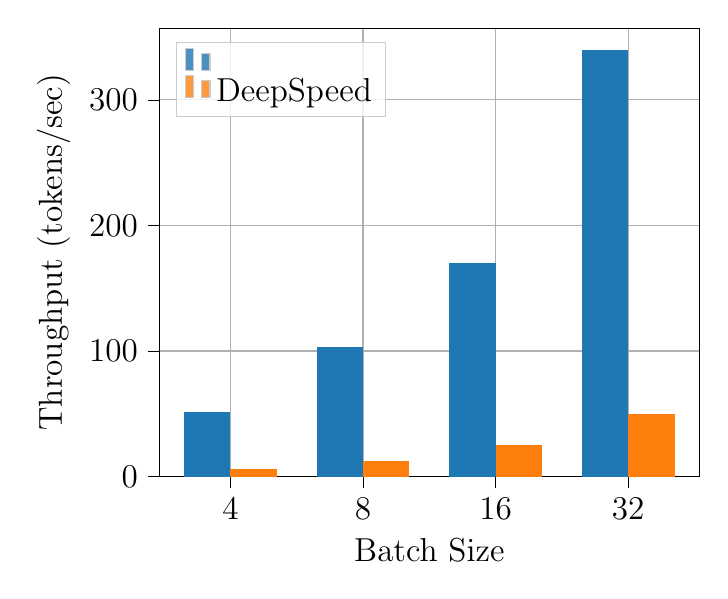
\begin{tikzpicture}

  \definecolor{darkgray176}{RGB}{176,176,176}
  \definecolor{darkorange25512714}{RGB}{255,127,14}
  \definecolor{lightgray204}{RGB}{204,204,204}
  \definecolor{steelblue31119180}{RGB}{31,119,180}
  
  \begin{axis}[
    title style={font=\Large},
    label style={font=\large},
    tick label style={font=\large},
    legend style={font=\large},
  legend cell align={left},
  legend style={
    fill opacity=0.8,
    draw opacity=1,
    text opacity=1,
    at={(0.03,0.97)},
    anchor=north west,
    draw=lightgray204
  },
  tick align=outside,
  tick pos=left,
  % title={Throughput Comparison: \sys vs DeepSpeed},
  x grid style={darkgray176},
  xlabel={Batch Size},
  xmajorgrids,
  xmin=-0.36, xmax=3.71,
  xtick style={color=black},
  xtick={0.175,1.175,2.175,3.175},
  xticklabels={4,8,16,32},
  y grid style={darkgray176},
  ylabel={Throughput (tokens/sec)},
  ymajorgrids,
  ymin=0, ymax=357,
  ytick style={color=black}
  ]
  \draw[draw=none,fill=steelblue31119180] (axis cs:-0.175,0) rectangle (axis cs:0.175,51.54);
  \addlegendimage{ybar,ybar legend,draw=none,fill=steelblue31119180}
  \addlegendentry{\sys}
  
  \draw[draw=none,fill=steelblue31119180] (axis cs:0.825,0) rectangle (axis cs:1.175,103);
  \draw[draw=none,fill=steelblue31119180] (axis cs:1.825,0) rectangle (axis cs:2.175,170);
  \draw[draw=none,fill=steelblue31119180] (axis cs:2.825,0) rectangle (axis cs:3.175,340);
  \draw[draw=none,fill=darkorange25512714] (axis cs:0.175,0) rectangle (axis cs:0.525,6.26);
  \addlegendimage{ybar,ybar legend,draw=none,fill=darkorange25512714}
  \addlegendentry{DeepSpeed}
  
  \draw[draw=none,fill=darkorange25512714] (axis cs:1.175,0) rectangle (axis cs:1.525,12.52);
  \draw[draw=none,fill=darkorange25512714] (axis cs:2.175,0) rectangle (axis cs:2.525,25);
  \draw[draw=none,fill=darkorange25512714] (axis cs:3.175,0) rectangle (axis cs:3.525,50);
  \end{axis}
  
  \end{tikzpicture}
   % 插入 TikZ 图
 }
    \caption{Throughput of \sys and \deepspeed with varying batch sizes. Model: Qwen2-beta-7B}
    \label{fig:moti1c}
\end{figure}


Unfortunately, for most modern LLMs, the computation 
is much shorter than the transfer time of a layer. 
%
We demonstrate this in Figure~\ref{fig:moti1} (b), where the transfer time is 3.5\X and 13.8\X longer than the computation time for the prefill and decoding phase, respectively. 
%
As a result, as shown in Figure~\ref{fig:moti1} (a), \deepspeed increases the
serving latency by up to 9.5\X, resulting in frequent SLO violations for all evaluated models. 
%
In addition to latency, since the GPU waits for the data most of the time, 
such an approach also reduces throughput by up to 8.2\X, as shown in Figure~\ref{fig:moti1c}. 

This is a major limitation since, for many user-facing LLM tasks, such as those discussed in \S\ref{sec:slo}, meeting the latency SLO is the top priority. 
%
Even a single SLO violation incurs a severe economic loss, thus defeating the purpose of minimizing operational costs in offloading approaches. 
%
Therefore, \deepspeed is limited to only those LLM tasks that do not require human interactions. 


\noindent \textbf{Obvervation \#1: Keeping only one layer in GPU, as done by \deepspeed, 
is prone to severe SLO violations.}




%-------------------------------------------------------------------------------

\subsection{Estimating Execution Time}
\label{sec:estimating}



As discussed in \S\ref{sec:prior}, the optimization goal of \flexgen is to 
maximize serving throughput. 
%
To evaluate \flexgen in our target scenario, we made a slight modification to 
the decision algorithm in \flexgen: it now takes a target SLO as input 
and output maximum offloaded portion. 
%
We verify that this modified, SLO-aware version of \flexgen functions correctly and can successfully meet the specified SLOs. 
%
For simplicity, we uses \flexgen to refer to this modified version throughout the rest of the paper. 

We found that a fundamental limitation of \flexgen is that it decides 
the offloaded portion~(\S\ref{sec:prior}) statically~(before 
the requests are actually executed); 
in other words, \flexgen cannot adjust the offloaded portion during execution based on current system status. 
%
Therefore, to avoid SLO violations, with \flexgen, one has to conservatively estimate for the worst case, making \flexgen underutilize host memory but rather uses much more GPU memory than necessary. 
%
As a result, \flexgen often fails to achieve the optimal performance, as shown in Figure~\ref{fig:moti2b}.  
%
The SLO is the TPOT when running without offloading. 
%
In this case, \flexgen uses 2.1\X less host memory than \sys, and thus supports smaller batch sizes, leading to 1.9\X throughput reduction. 
%
We note that this is the best case for \flexgen and a more relaxed SLO 
makes the throughput difference even larger. 

With \flexgen, an important factor for underutilizing host memory is that \flexgen statically estimates serving latency using peak GPU performance. 
%
This is necessary to avoid SLO violations since the estimated value is the theoretical lower bound of the serving latency. 
%
However, as shown in Figure~\ref{fig:moti2}, the estimated latency  
is much shorter than the real one. 
%
This makes \flexgen offload a smaller amount of model state than is necessary to host memory, since \flexgen mistakenly believes that 
the computation time is not long enough to overlap the transfer time of the larger
model state. 

\begin{figure}[t]
    \centering
    \resizebox{\columnwidth}{!}{
        % This file was created with tikzplotlib v0.10.1.
\begin{tikzpicture}

    \definecolor{darkgray176}{RGB}{176,176,176}
    \definecolor{green}{RGB}{0,128,0}
    \definecolor{lightgray204}{RGB}{204,204,204}
    
    \begin{groupplot}[group style={group size=2 by 1, horizontal sep=2cm},
      title style={font=\Large},
    label style={font=\large},
    tick label style={font=\large},
    legend style={font=\large}]
      \nextgroupplot[
        legend cell align={left},
        legend style={
          fill opacity=0.8,
          draw opacity=1,
          text opacity=1,
          at={(0.03,0.97)},
          anchor=north west,
          draw=lightgray204
        },
        tick align=outside,
        tick pos=left,
        title={(a) Sequence Length = 512},
        x grid style={darkgray176},
        xlabel={Batch Size},
        xmajorgrids,
        xmin=-1.1, xmax=67.1,
        xtick style={color=black},
        y grid style={darkgray176},
        ylabel={Latency (ms)},
        ymajorgrids,
        ymin=10.3955, ymax=142.7145,
        ytick style={color=black}
        ]
        \addplot [semithick, blue, dashed, mark=*, mark size=3, mark options={solid}]
        table {%
        2 16.41
        4 18.091
        8 21.79
        16 30.277
        32 49.604
        64 84.493
        };
        \addlegendentry{Estimated}
        \addplot [semithick, green, mark=triangle*, mark size=3, mark options={solid}]
        table {%
        2 32.85
        4 36.17
        8 42.91
        16 56.72
        32 83.74
        64 136.7
        };
        \addlegendentry{Actual}
        
        \nextgroupplot[
        legend cell align={left},
        legend style={fill opacity=0.8, draw opacity=1, text opacity=1, draw=lightgray204},
        scaled y ticks=manual:{}{\pgfmathparse{#1}},
        tick align=outside,
        tick pos=left,
        title={(b) Batch Size = 16},
        x grid style={darkgray176},
        xlabel={Sequence Length},
        xmajorgrids,
        xmin=16, xmax=1072,
        xtick style={color=black},
        y grid style={darkgray176},
        ylabel={Latency (ms)},
        ymajorgrids,
        ymin=10.3955, ymax=142.7145,
        ytick style={color=black},
        ]
        \addplot [semithick, blue, dashed, mark=*, mark size=3, mark options={solid}]
        table {%
        64 17.043
        128 18.709
        256 21.87
        512 29.08
        1024 49.196
        };
        \addlegendentry{Estimated}
        \addplot [semithick, green, mark=triangle*, mark size=3, mark options={solid}]
        table {%
        64 33.04
        128 36.06
        256 42.54
        512 56.72
        1024 87.42
        };
        \addlegendentry{Actual}
        \end{groupplot}
        
        \end{tikzpicture}
         % 插入 TikZ 图
 }
    \caption{The actual serving latency vs. the one estimated by \flexgen. Model: OPT-13B.
 }
    \label{fig:moti2}
\end{figure}

\begin{figure}[t]
    \centering
    \resizebox{\columnwidth}{!}{
        % This file was created with tikzplotlib v0.10.1.
\begin{tikzpicture}

  \definecolor{darkgray176}{RGB}{176,176,176}
  \definecolor{darkorange25512714}{RGB}{255,127,14}
  \definecolor{steelblue31119180}{RGB}{31,119,180}
  
  \begin{groupplot}[group style={group size=2 by 1, horizontal sep=2cm},
    title style={font=\Large},
    label style={font=\large},
    tick label style={font=\large},
    legend style={font=\large}]
  \nextgroupplot[
  legend cell align={left},
  legend style={
    fill opacity=0.8,
    draw opacity=1,
    text opacity=1,
    at={(0.03,0.97)},
    anchor=north west,
    draw=none
  },
  tick align=outside,
  tick pos=left,
  title={(a) Memory Usage on Offloading Devices},
  x grid style={darkgray176},
  xlabel={Batch Size},
  xmin=-0.38, xmax=1.38,
  xtick style={color=black},
  xtick={0,1},
  xticklabels={8,32},
  y grid style={darkgray176},
  ylabel={Memory Usage (GB)},
  ymin=0, ymax=12.5685,
  ytick style={color=black}
  ]
  \draw[draw=none,fill=steelblue31119180] (axis cs:-0.3,0) rectangle (axis cs:0,7.77);
  \addlegendimage{ybar,ybar legend,draw=none,fill=steelblue31119180}
  \addlegendentry{\sys}
  
  \draw[draw=none,fill=steelblue31119180] (axis cs:0.7,0) rectangle (axis cs:1,11.97);
  \draw[draw=none,fill=darkorange25512714] (axis cs:2.77555756156289e-17,0) rectangle (axis cs:0.3,4.8);
  \addlegendimage{ybar,ybar legend,draw=none,fill=darkorange25512714}
  \addlegendentry{FlexGen}
  
  \draw[draw=none,fill=darkorange25512714] (axis cs:1,0) rectangle (axis cs:1.3,5.57);
  \draw (axis cs:-0.2,7.97) node[
    scale=0.5,
    anchor=base,
    text=black,
    rotate=0.0
  ]{7.77};
  \draw (axis cs:0.8,12.17) node[
    scale=0.5,
    anchor=base,
    text=black,
    rotate=0.0
  ]{11.97};
  \draw (axis cs:0.2,5) node[
    scale=0.5,
    anchor=base,
    text=black,
    rotate=0.0
  ]{4.80};
  \draw (axis cs:1.2,5.77) node[
    scale=0.5,
    anchor=base,
    text=black,
    rotate=0.0
  ]{5.57};
  
  \nextgroupplot[
  legend cell align={left},
  legend style={
    fill opacity=0.8,
    draw opacity=1,
    text opacity=1,
    at={(0.03,0.97)},
    anchor=north west,
    draw=none
  },
  tick align=outside,
  tick pos=left,
  title={(b) Throughput Comparison},
  x grid style={darkgray176},
  xlabel={Batch Size},
  xmin=-0.38, xmax=1.38,
  xtick style={color=black},
  xtick={0,1},
  xticklabels={8,32},
  y grid style={darkgray176},
  ylabel={Throughput (tokens/s)},
  ymin=0, ymax=59.997,
  ytick style={color=black}
  ]
  \draw[draw=none,fill=steelblue31119180] (axis cs:-0.3,0) rectangle (axis cs:0,21.97);
  \draw[draw=none,fill=steelblue31119180] (axis cs:0.7,0) rectangle (axis cs:1,57.14);
  \draw[draw=none,fill=darkorange25512714] (axis cs:2.77555756156289e-17,0) rectangle (axis cs:0.3,11.85);
  \draw[draw=none,fill=darkorange25512714] (axis cs:1,0) rectangle (axis cs:1.3,35.46);
  \draw (axis cs:-0.2,23.97) node[
    scale=0.5,
    anchor=base,
    text=black,
    rotate=0.0
  ]{21.97};
  \draw (axis cs:0.8,59.14) node[
    scale=0.5,
    anchor=base,
    text=black,
    rotate=0.0
  ]{57.14};
  \draw (axis cs:0.2,13.85) node[
    scale=0.5,
    anchor=base,
    text=black,
    rotate=0.0
  ]{11.85};
  \draw (axis cs:1.2,37.46) node[
    scale=0.5,
    anchor=base,
    text=black,
    rotate=0.0
  ]{35.46};
  \end{groupplot}
  
  \end{tikzpicture}
   % 插入 TikZ 图
 }
    \caption{Comparison of \sys and FlexGen in (a) Memory usage on the offloading devices and (b) Throughput. Model: OPT-13B.}
    \label{fig:moti2b}
\end{figure}



\noindent \textbf{Obvervation \#2: Estimating model execution time 
using peak GPU performance, as with \deepspeed, is inaccurate and 
heavily underutilizes host memory.}



%-------------------------------------------------------------------------------

\subsection{Bandwidth Contention}
\label{sec:bandwidth}

Another important factor for \flexgen to underutilize host memory is 
the contention on transfer bandwidth between host and GPU memory. 
%
Specifically, to minimize operational costs, the current industry practice is to place multiple GPUs on a single machine node. 
%a
However, some of these GPUs share a single PCIe bus~(which connects the host and GPUs), and thus contends for the PCIe bandwidth~\cite{pciecontention, pciecontention2}. 
% cite some papers on the PCIe contention caused by GPUs. 
%
As a result, the available bandwidth to transfer LLM state for each 
individual GPU fluctuates during serving a request. 

With \flexgen, in the presence of bandwidth contention, to meet SLO, 
one must again estimate the worst case:  
%
each GPU only gets $1/n$ of the bandwidth, where $n$ is the number of GPUs that share a PCIe bus.  
%
However, for a given GPU, the available bandwidth may fluctuate but is often much larger than the worst-case one, since other GPUs may be idle, or do not 
fully utilize their share of the bandwidth. 
%
As a result, \flexgen overestimates the transfer time, again offloading a smaller amount of LLM state than is necessary to host memory. 



\noindent \textbf{Observation \#3: \flexgen statically estimates the PCIe bandwidth under contention, thereby underutilizing the host memory.}

